\documentclass[11pt,a4paper]{article}
\usepackage[utf8]{inputenc}
\usepackage{graphicx}
\usepackage{geometry}
\usepackage{listings}
\usepackage{xcolor}
\usepackage{fancyhdr}
\usepackage{titlesec}
\usepackage{url}

% Page setup
\geometry{left=2cm,right=2cm,top=2.5cm,bottom=2.5cm}
\pagestyle{fancy}
\fancyhf{}
\rhead{FIT5032 Assessed Lab 5}
\lhead{Vue.js Router Implementation}
\cfoot{\thepage}

% Code listing style
\lstset{
    basicstyle=\footnotesize\ttfamily,
    breaklines=true,
    frame=single,
    numbers=left,
    numberstyle=\tiny,
    showstringspaces=false,
    commentstyle=\color{gray},
    keywordstyle=\color{blue},
    stringstyle=\color{red},
    escapeinside={(*@}{@*)}
}

\title{\textbf{FIT5032 Assessed Lab 5 Submission\\Vue.js Router and Authentication Implementation}}
\author{Student Name: [Du Daoan]\\Student ID: [35523166]}
\date{}

\begin{document}

\maketitle


% =============================================================================
% EFOLIO TASK 5.1 (PASS AND CREDIT LEVEL)
% =============================================================================

\section{EFOLIO TASK 5.1 - Password Confirmation Validation}

\subsection{Screenshot 1: Password Confirmation Validation Error}

% Password validation error screenshot
 \begin{figure}[h]
     \centering
     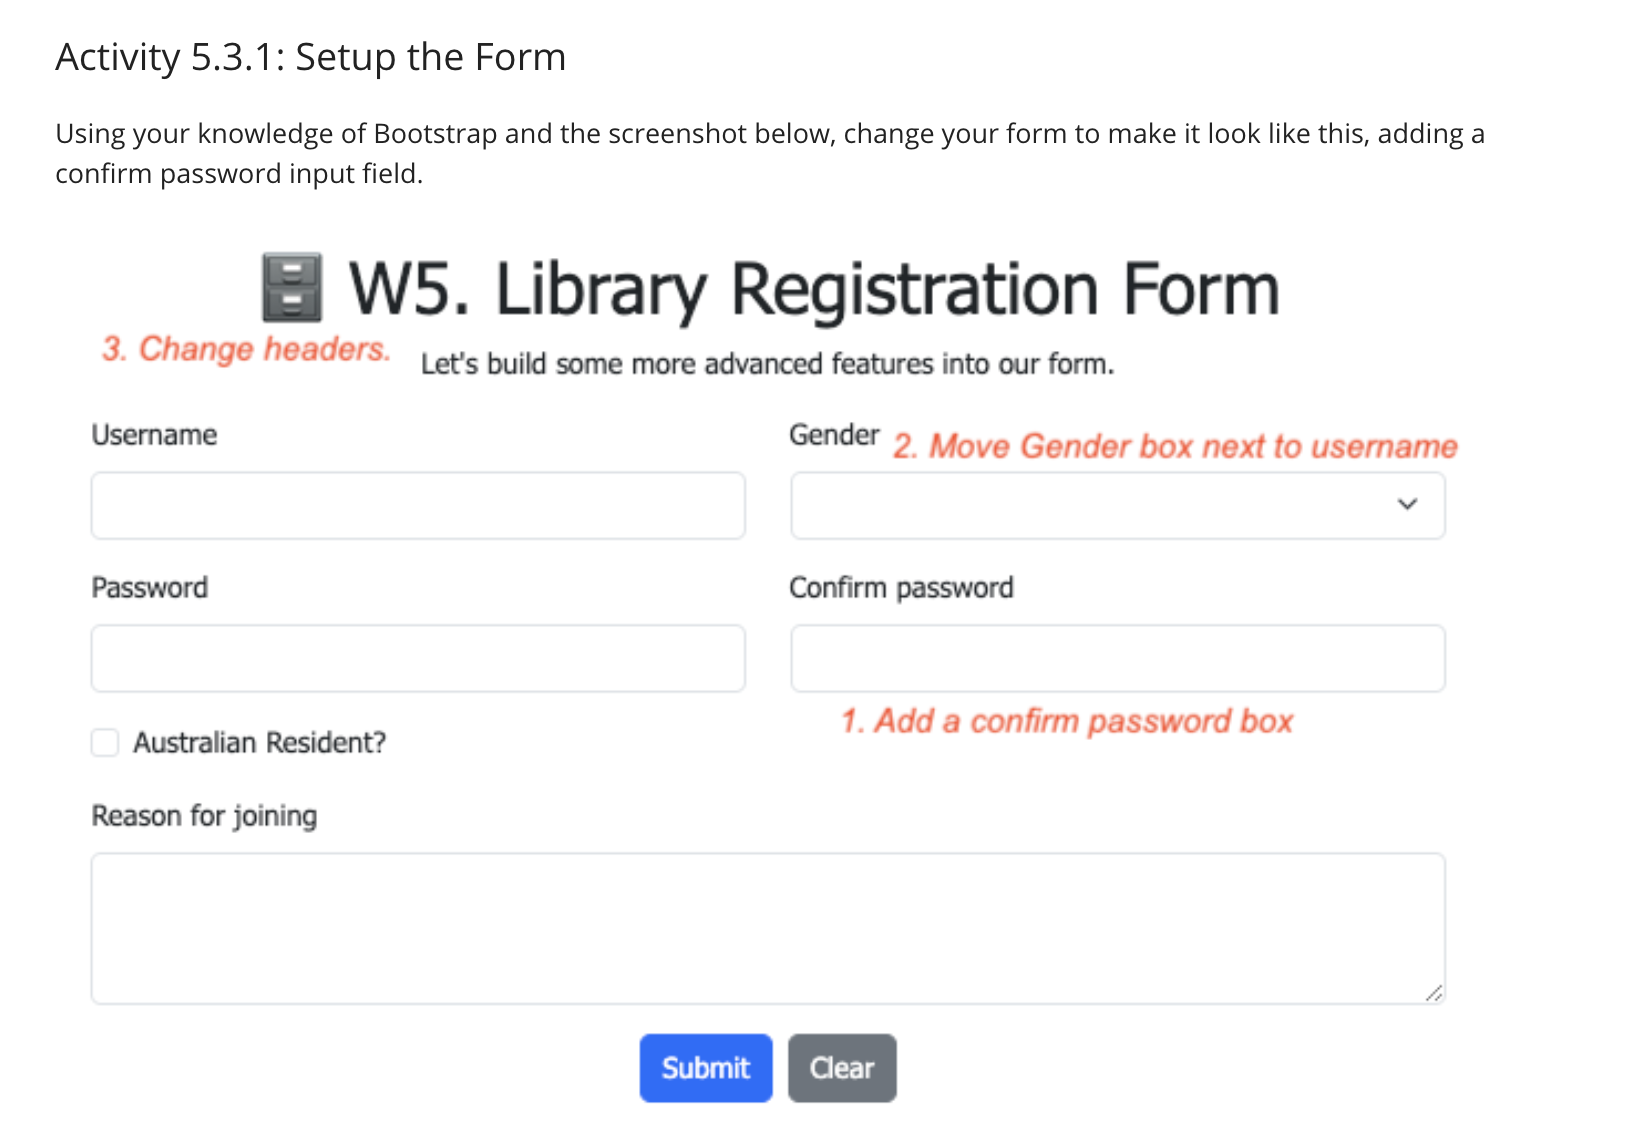
\includegraphics[width=0.9\textwidth]{password_validation_error.png}
     \caption{Password confirmation validation showing error message when passwords do not match}
     \label{fig:password_error}
\end{figure}

\textbf{Evidence Required:} Screenshot showing error message when passwords do not match.

\subsection{Screenshot 2: VueJS DevTools Testing}

% VueJS DevTools screenshot
\begin{figure}[h]
     \centering
     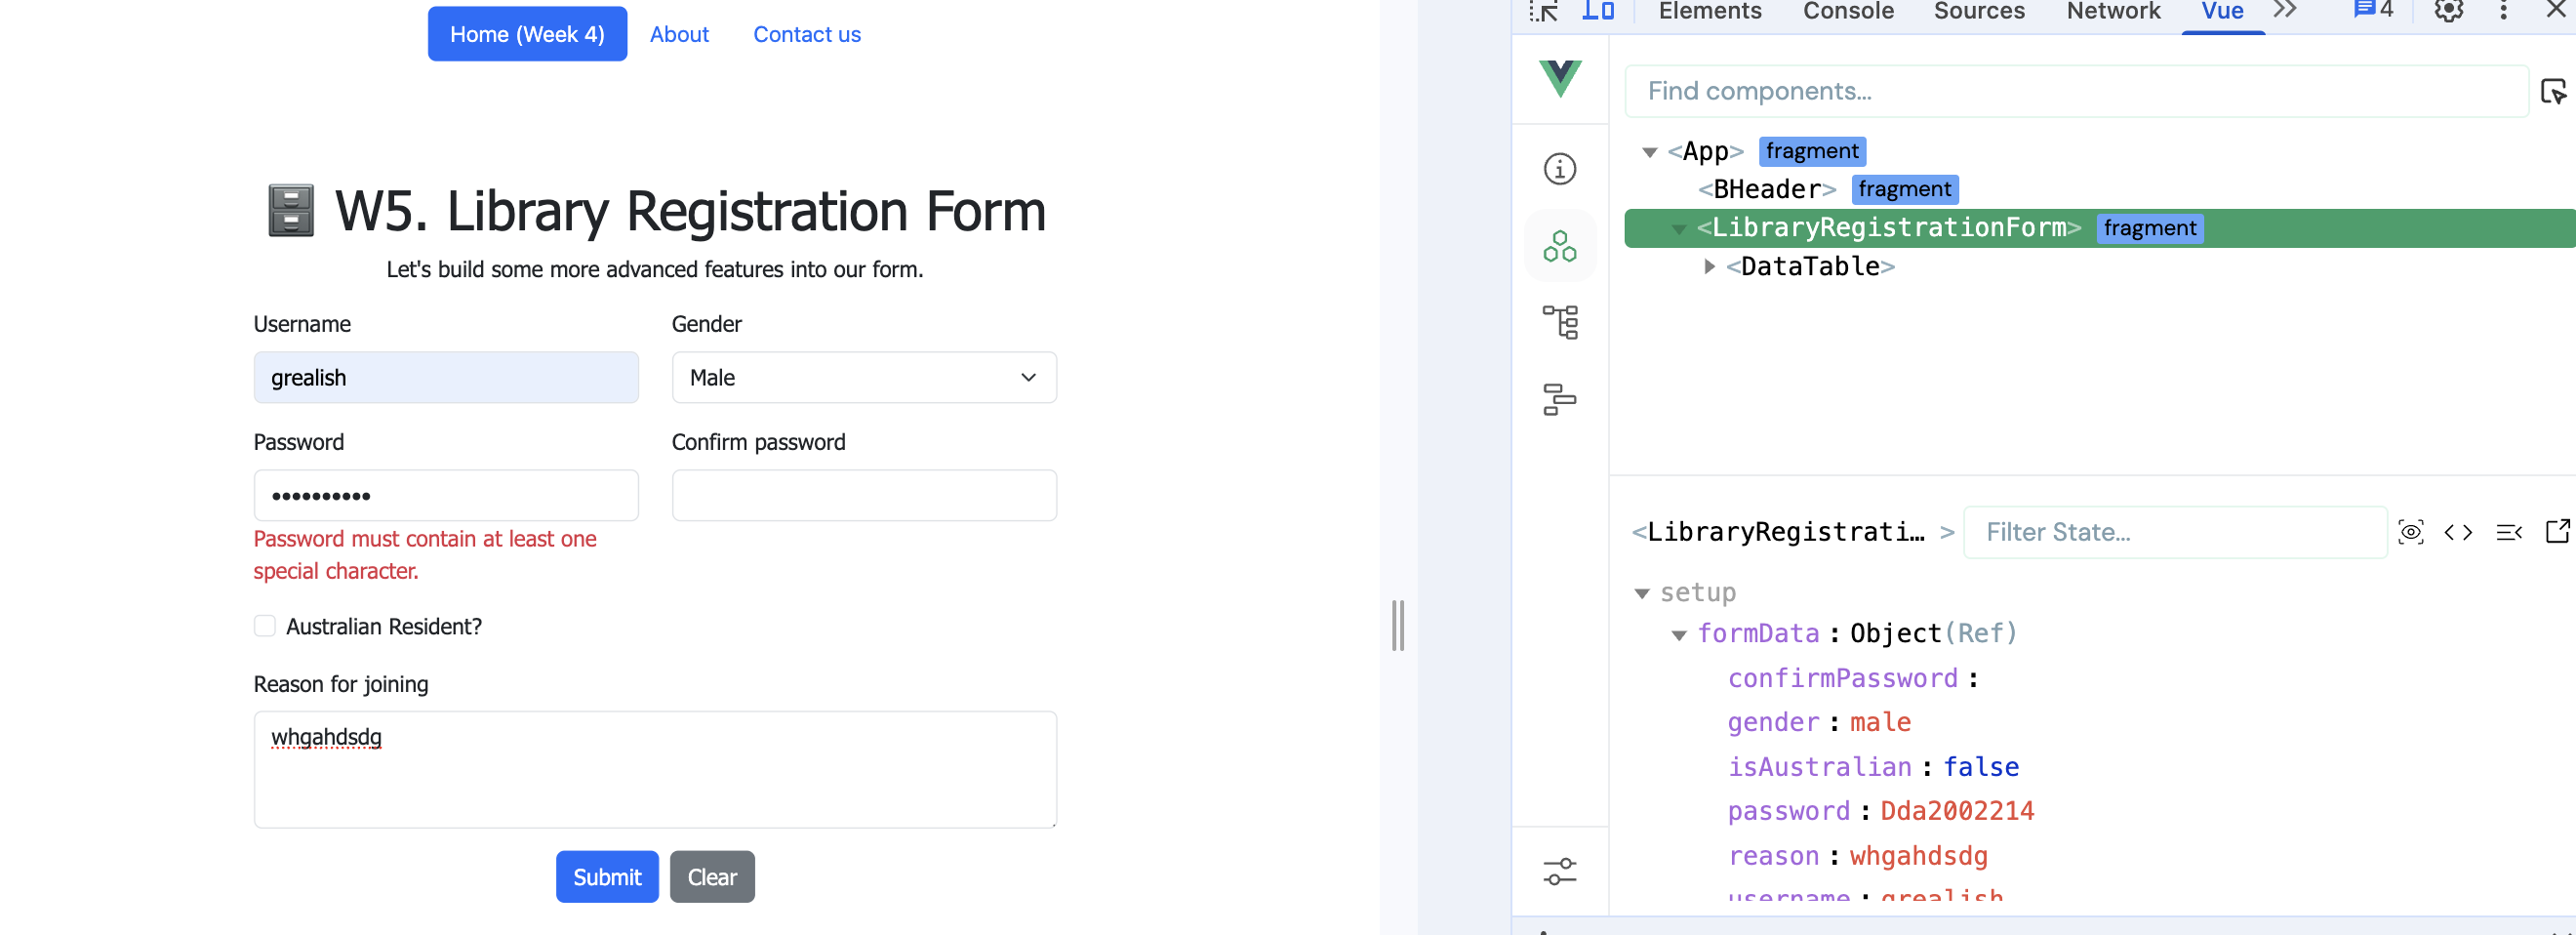
\includegraphics[width=0.9\textwidth]{vue_devtools_testing.png}
     \caption{Using VueJS DevTools to test components and debug application}
     \label{fig:vue_devtools}
\end{figure}

\textbf{Evidence Required:} Screenshot demonstrating knowledge of VueJS DevTools for debugging/testing.

\newpage

% =============================================================================
% EFOLIO TASK 5.2 (DISTINCTION AND HD LEVEL)
% =============================================================================

\section{EFOLIO TASK 5.2 - Advanced Router Implementation}

\subsection{File: router/index.js}

\begin{lstlisting}[caption=Router configuration with navigation guards]
import { createRouter, createWebHistory } from 'vue-router'
import HomeView from '../views/HomeView.vue'
import AboutView from '../views/AboutView.vue'
import LoginView from '../views/LoginView.vue'
import AccessDeniedView from '../views/AccessDeniedView.vue'
import { checkAuth } from '../auth.js'

const routes = [
  {
    path: '/',
    name: 'Home',
    component: HomeView
  },
  {
    path: '/about',
    name: 'About',
    component: AboutView,
    meta: { requiresAuth: true }
  },
  {
    path: '/login',
    name: 'Login',
    component: LoginView
  },
  {
    path: '/access-denied',
    name: 'AccessDenied',
    component: AccessDeniedView
  }
]

const router = createRouter({
  history: createWebHistory(),
  routes
})

router.beforeEach((to, from, next) => {
  if (to.matched.some(record => record.meta.requiresAuth)) {
    if (!checkAuth()) {
      next({
        path: '/access-denied',
        query: { redirect: to.fullPath }
      })
    } else {
      next()
    }
  } else {
    next()
  }
})

export default router
\end{lstlisting}

\newpage

\subsection{File: src/App.vue}

\begin{lstlisting}[caption=Main App component with router-view]
<script setup>
import BHeader from './components/BHeader.vue'
</script>

<template>
  <header>
    <BHeader />
  </header>
  <main>
    <router-view></router-view>
  </main>
</template>

<style>
.container {
  font-family: 'Segoe UI', Tahoma, Geneva, Verdana, sans-serif;
  max-width: 80vw;
  margin: 0 auto;
  padding: 20px;
  border-radius: 10px;
}

.card {
  border: 1px solid #ccc;
  border-radius: 10px;
  box-shadow: 0 2px 4px rgba(0, 0, 0, 0.1);
}

.card-header {
  background-color: #275fda;
  color: white;
  padding: 10px;
  border-radius: 10px 10px 0 0;
}
</style>
\end{lstlisting}

\newpage

\subsection{File: src/views/HomeView.vue}

\begin{lstlisting}[caption=Home view with registration form]
<script setup>
import { ref } from 'vue'
import DataTable from 'primevue/datatable'
import Column from 'primevue/column'

const formData = ref({
  username: '',
  password: '',
  confirmPassword: '',
  isAustralian: false,
  reason: '',
  gender: ''
})

const validateConfirmPassword = (blur) => {
  if (formData.value.confirmPassword !== formData.value.password) {
    if (blur) errors.value.confirmPassword = 'Passwords do not match'
  } else {
    errors.value.confirmPassword = null
  }
}

const validateReason = () => {
  const reason = formData.value.reason.toLowerCase()
  if (reason.includes('friend')) {
    errors.value.reason = { 
      type: 'success', 
      message: 'Great to have a friend' 
    }
  } else {
    errors.value.reason = null
  }
}
</script>
\end{lstlisting}

\textbf{Key Features Implemented:}
\begin{itemize}
    \item Two-way data binding with v-model
    \item Form validation with real-time feedback
    \item Password confirmation validation
    \item Conditional rendering for success messages
\end{itemize}

\newpage

\subsection{Application Screenshots}

\subsubsection{Home Page Screenshot}

% Home page screenshot
\begin{figure}[h]
     \centering
     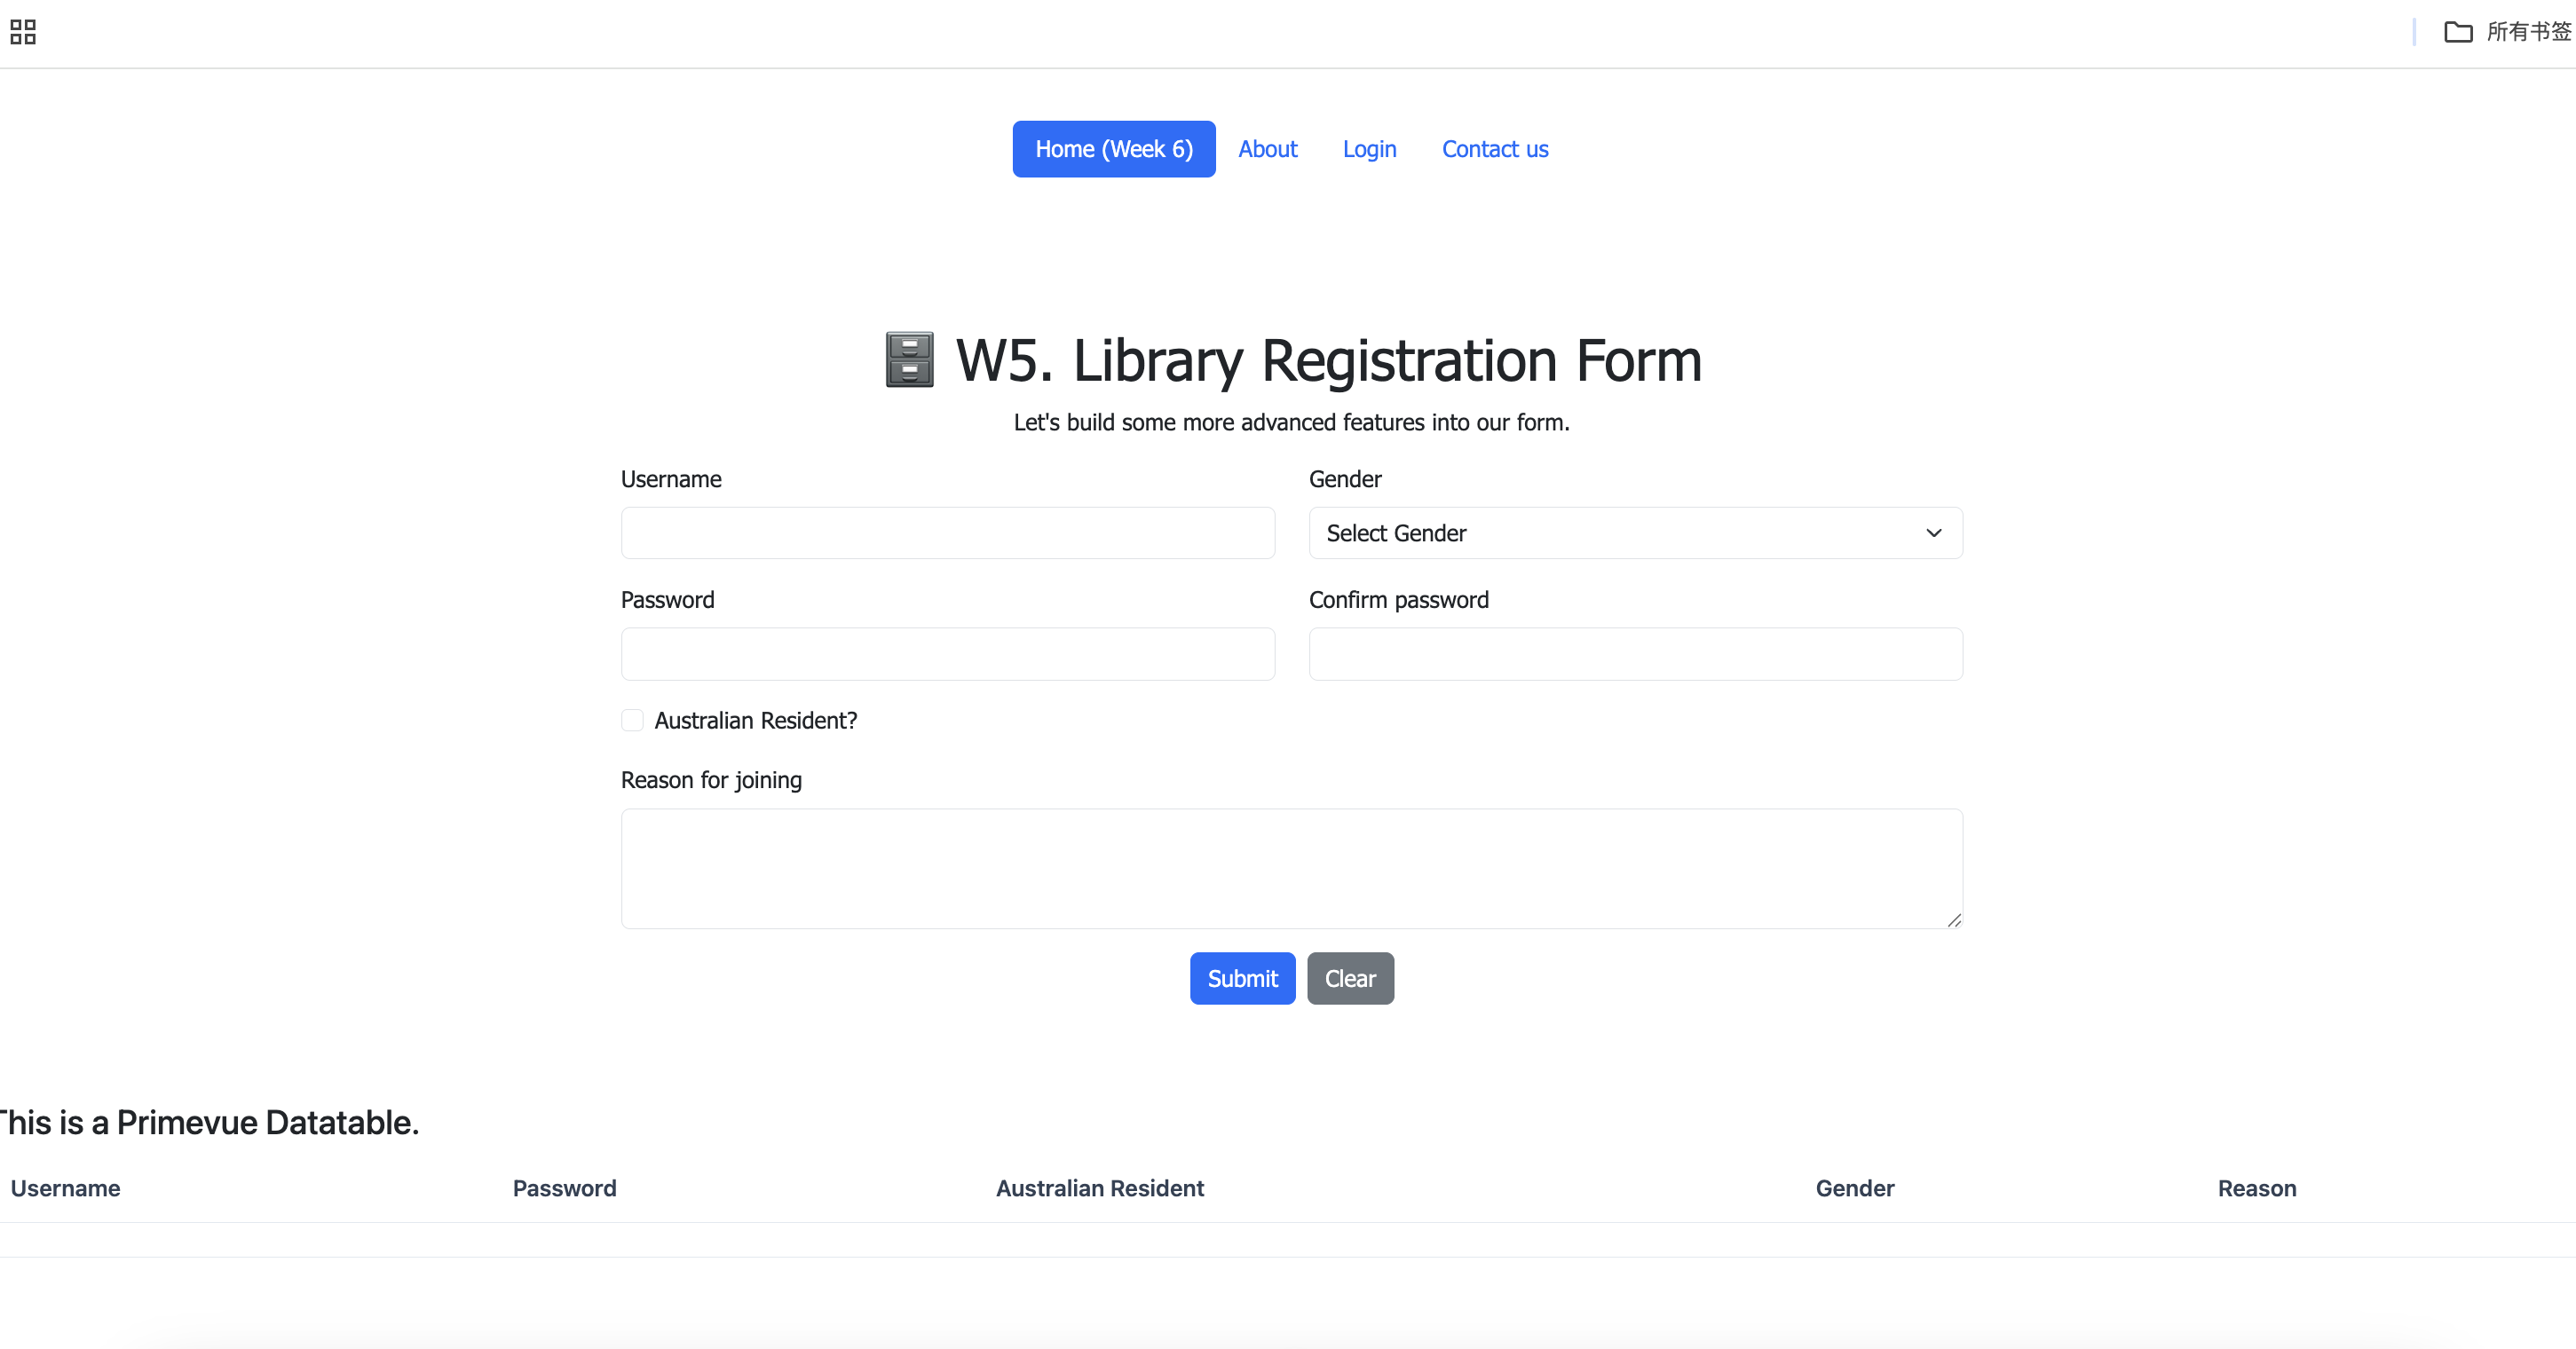
\includegraphics[width=0.9\textwidth]{home_page_localhost.png}
     \caption{Application running on localhost showing Home page with registration form}
     \label{fig:home_page}
\end{figure}

\textbf{Evidence Required:} Screenshot of application on localhost showing Home page.

\subsubsection{About Page Screenshot}

% About page screenshot
\begin{figure}[h]
     \centering
     
\includegraphics[width=0.9\textwidth]{about_page_localhost.png}
     \caption{Application showing About page (protected route for authenticated users)}
     \label{fig:about_page}
\end{figure}

\textbf{Evidence Required:} Screenshot of application showing About page navigation.

\newpage

\subsection{Custom Routing Screenshots}

\subsubsection{Login Page}

% Login page screenshot
 \begin{figure}[h]
     \centering
     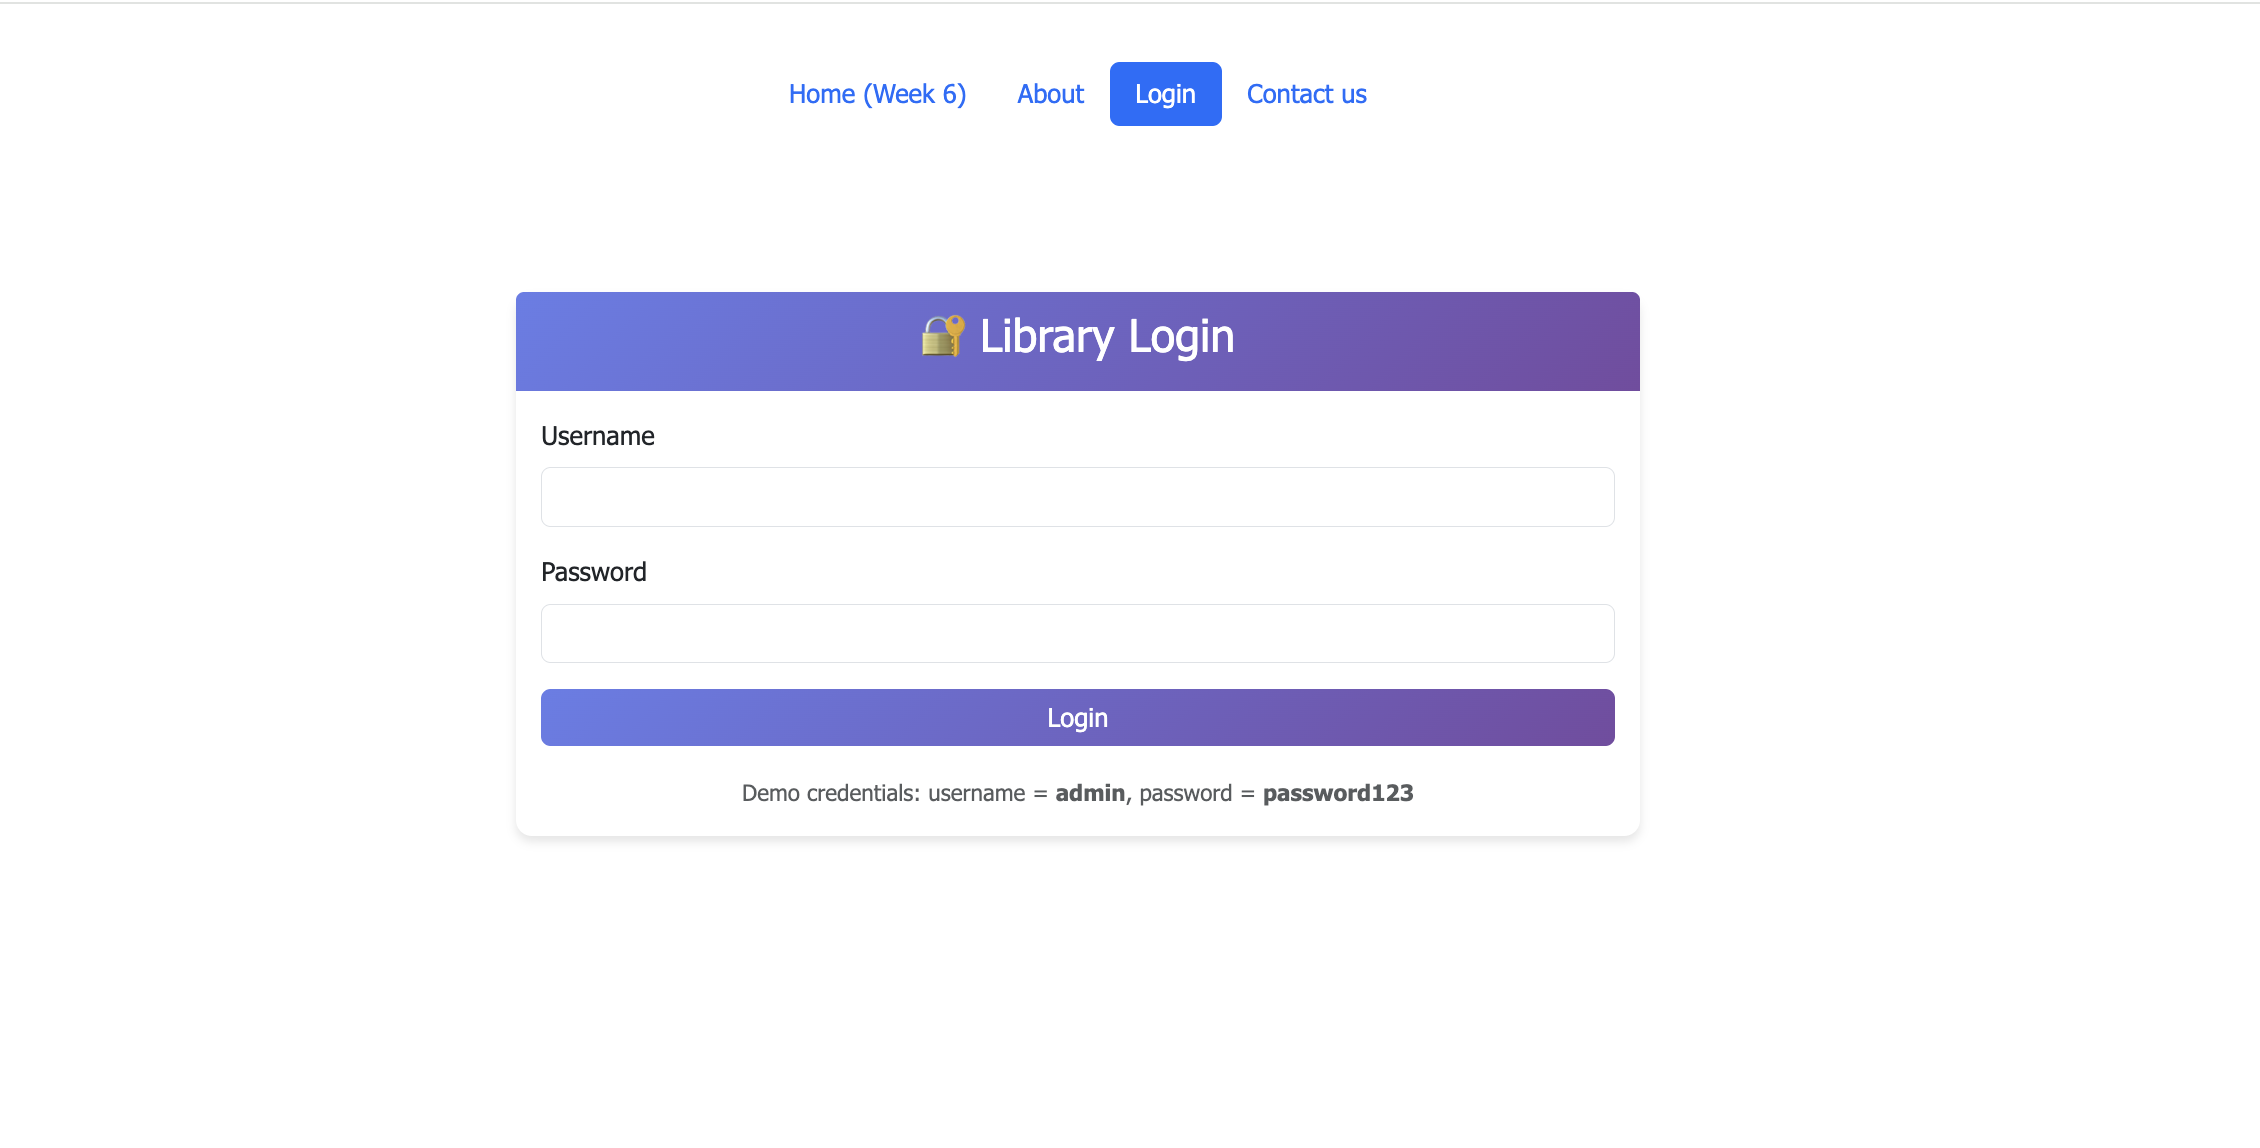
\includegraphics[width=0.9\textwidth]{login_page.png}
     \caption{Login page with authentication form}
     \label{fig:login_page}
\end{figure}

\subsubsection{Access Denied Page}

% Access denied screenshot
 \begin{figure}[h]
     \centering
     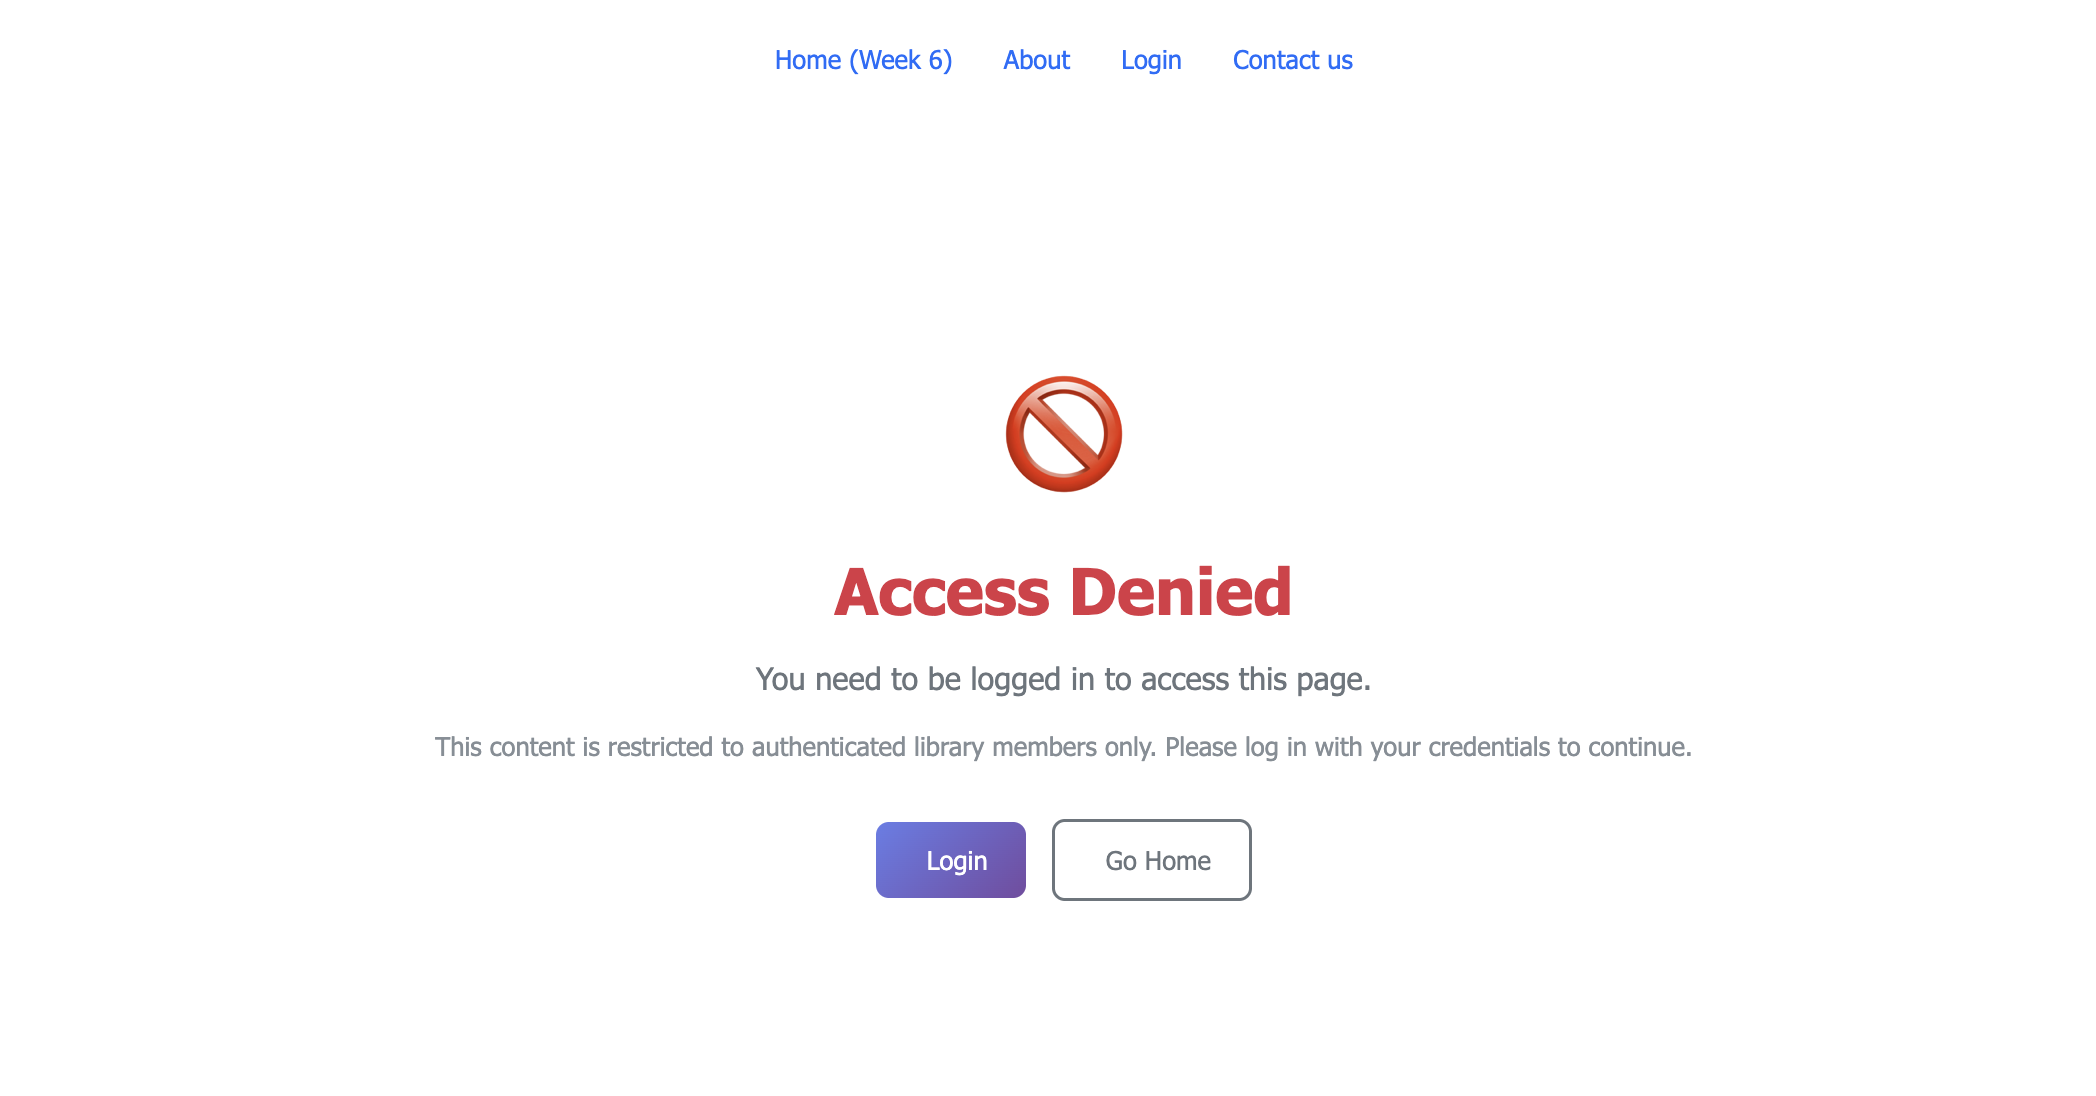
\includegraphics[width=0.9\textwidth]{access_denied_page.png}
     \caption{Access denied page shown to unauthenticated users}
     \label{fig:access_denied}
\end{figure}

\subsubsection{Navigation with Authentication State}

% Authentication navigation screenshot
\begin{figure}[h]
     \centering
     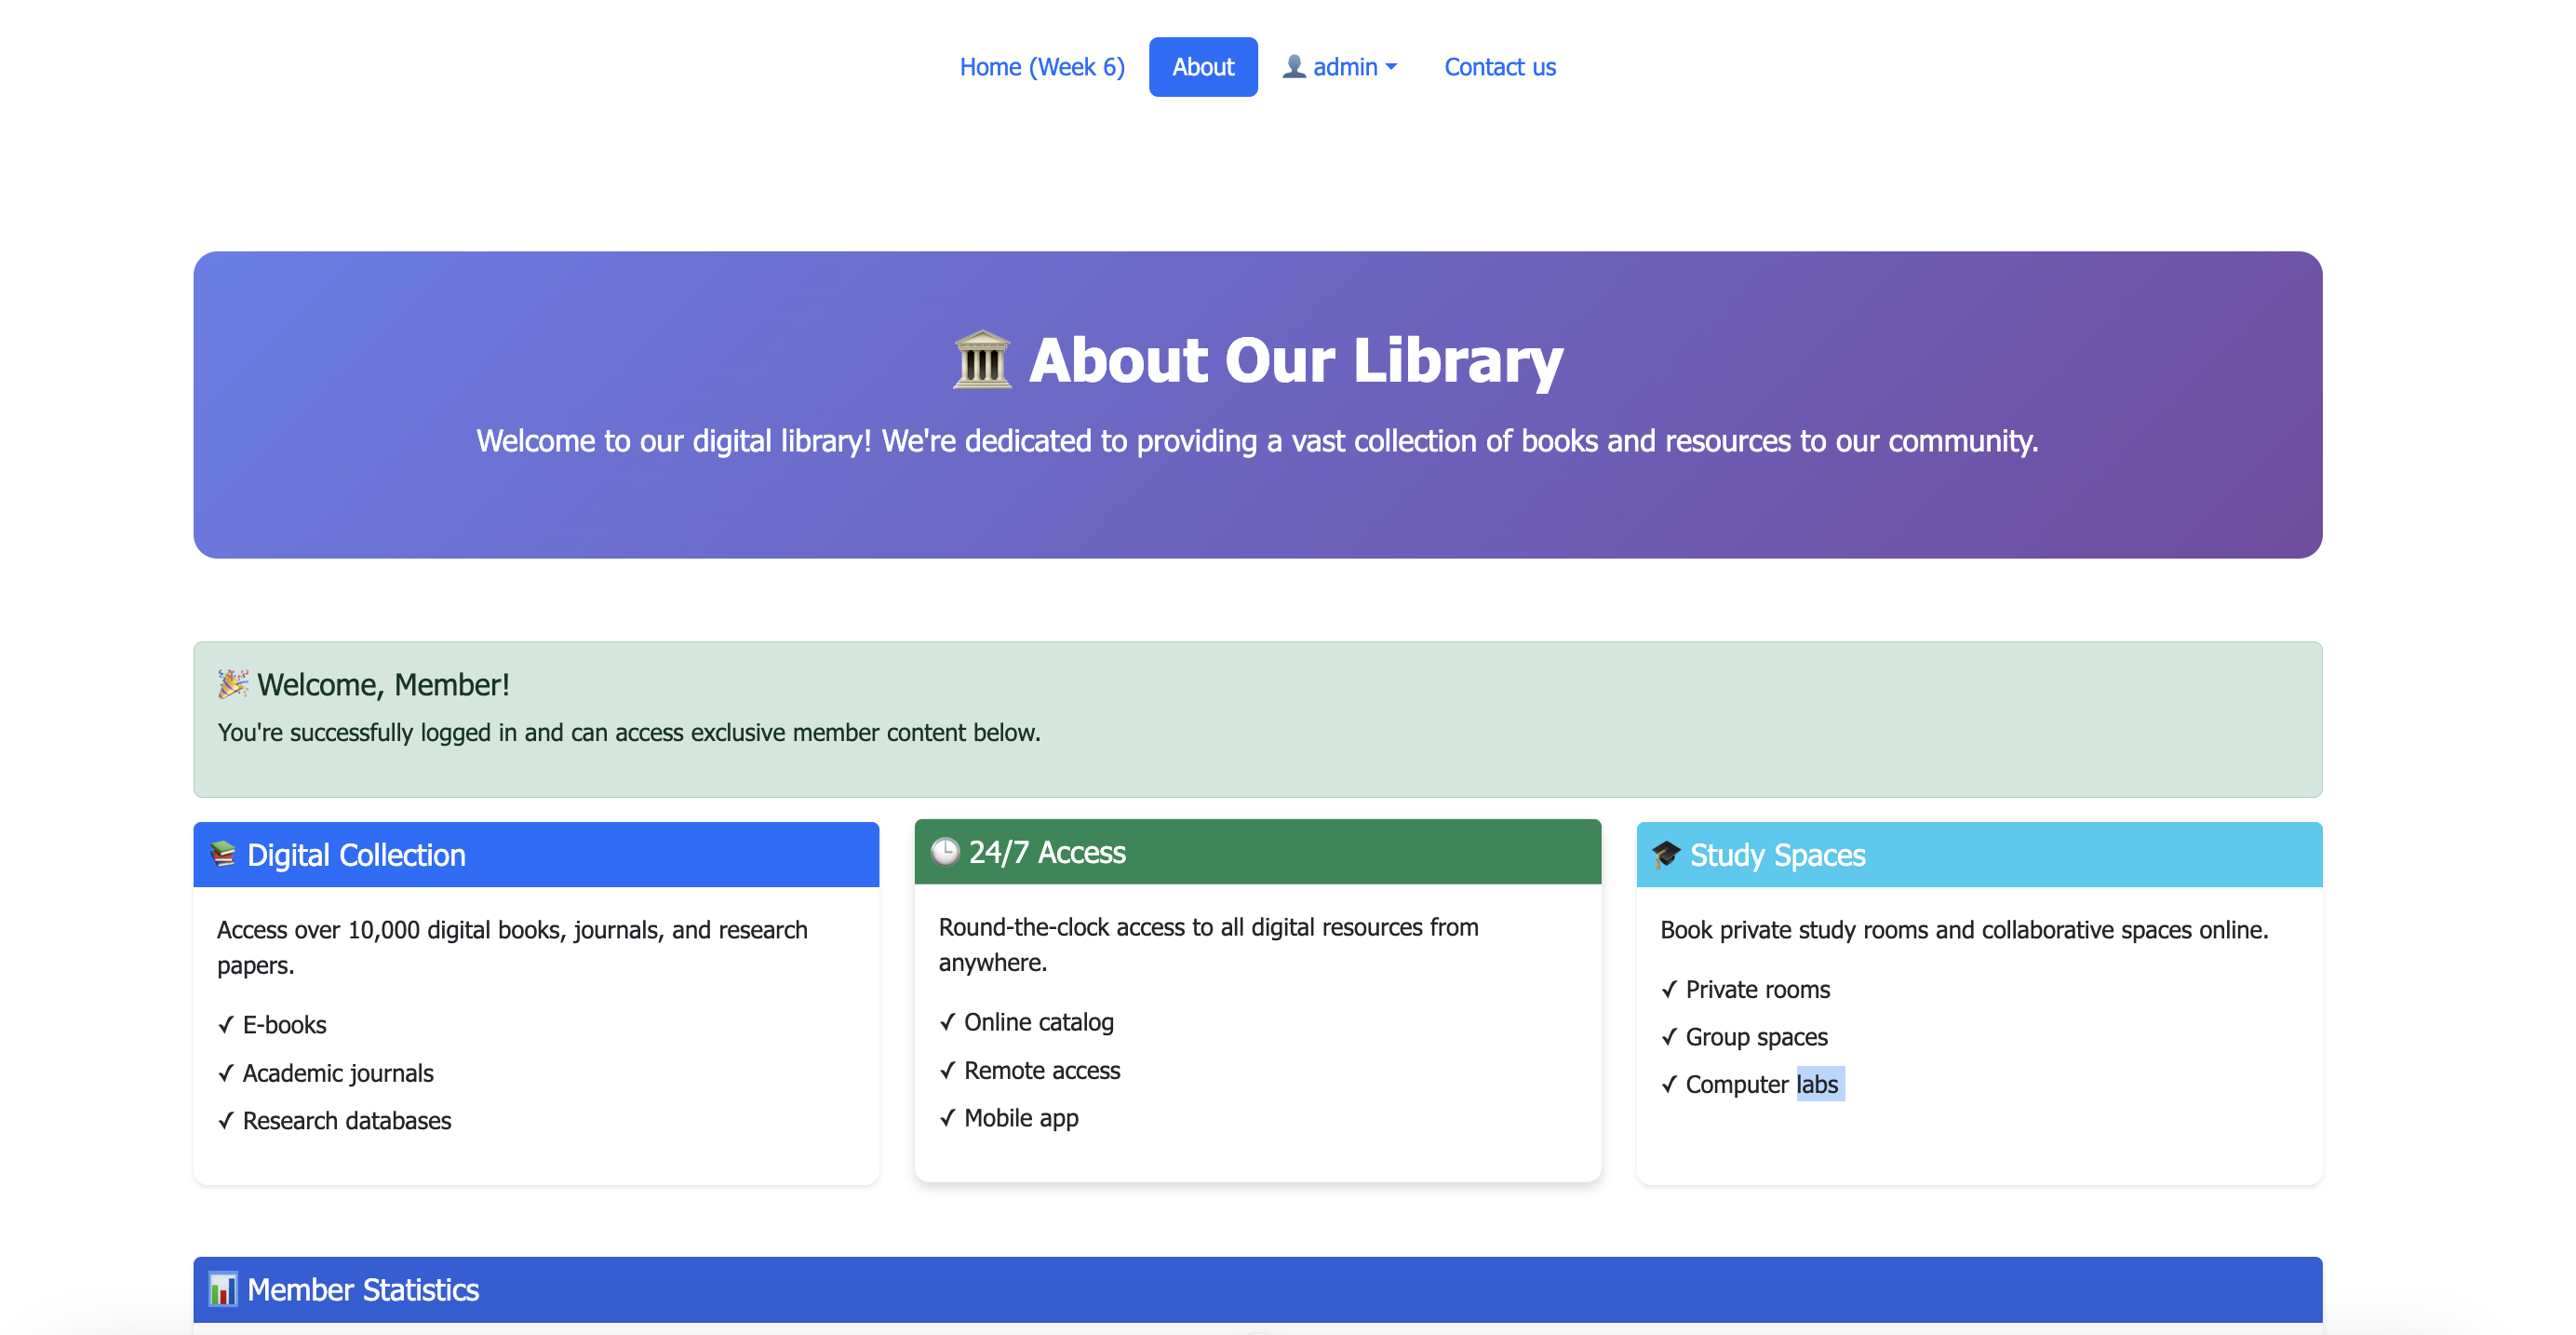
\includegraphics[width=0.9\textwidth]{authenticated_navigation.png}
     \caption{Navigation bar showing different options for authenticated users}
     \label{fig:auth_nav}
\end{figure}

\subsubsection{Route Protection in Action}

% Route protection screenshot
% \begin{figure}[h]
%     \centering
%     \includegraphics[width=0.9\textwidth]{route_protection.png}
%     \caption{Demonstration of route protection redirecting unauthenticated users}
%     \label{fig:route_protection}
% \end{figure}

\newpage

\section{Key Technical Achievements}

\subsection{Conditional Routing Implementation}
\begin{itemize}
    \item \textbf{Navigation Guards:} Implemented global beforeEach guard for route protection
    \item \textbf{Meta Fields:} Used route meta properties to mark protected routes
    \item \textbf{Authentication State:} Reactive authentication system using Vue 3 Composition API
    \item \textbf{Conditional Navigation:} Dynamic navigation menu based on user authentication status
\end{itemize}

\subsection{Security Features}
\begin{itemize}
    \item \textbf{Route Protection:} About page restricted to authenticated users only
    \item \textbf{Access Control:} Automatic redirection for unauthorized access attempts
    \item \textbf{Session Management:} Proper login/logout functionality
    \item \textbf{User Feedback:} Clear messaging for authentication states
\end{itemize}

\subsection{Advanced Vue.js Concepts Demonstrated}
\begin{itemize}
    \item \textbf{Composition API:} Used ref() for reactive state management
    \item \textbf{Router Integration:} Proper Vue Router 4 setup with history mode
    \item \textbf{Component Communication:} Shared authentication state across components
    \item \textbf{Conditional Rendering:} v-if/v-else for dynamic UI based on auth state
\end{itemize}

\section{Conclusion}

This implementation successfully demonstrates advanced Vue.js routing concepts including:
\begin{itemize}
    \item Conditional routing with navigation guards
    \item Route-based access control and security
    \item Dynamic navigation based on authentication state
    \item Industry-standard authentication patterns
    \item Proper separation of concerns in Vue.js architecture
\end{itemize}

The application provides a complete authentication workflow with secure routing, demonstrating mastery of Vue Router and modern Vue.js development practices.

\end{document} 